\section{Instalacja aplikacji}

Stopień trudności instalacji aplikacji zależny jest od typu procesora, na którym będzie uruchomiony nasz program oraz od tego, w jaki sposób chcemy jej używać. Należy mieć świadomość, że cały poniższy opis instalacji dotyczy przypadku 64-bitowego systemu Windows, jako platformy pod którą wymagane jest działanie aplikacji.

\subsection{Szybka instalacja}

Pliki binarne aplikacji zostały skompilowane przy użyciu kompilatora wbudowanego w Microsoft Visual Studio 2015. Sprawia to, że aplikacja korzysta z dodatkowych bibliotek dynamicznych, które musimy posiadać na komputerze, na którym uruchamiamy aplikacje. Gdy tego nie zrobimy, w trakcie uruchomienia dostaniemy komunikat o braku wymaganego pliku, taki jak poniżej.

TODO obrazek

Możemy dodać go, nie istalując powyższego środowiska, ale musimy być świadomi, że przy kolejnej próbie uruchomienia dostaniemy bliźniaczy komunikat dla innego pliku. Tak, więc rekomendowanym sposobem jest instalacja Microsoft Vistual Studio 2015, który zainstaluje wszystkie potrzebne biblioteki.

Drugą rzeczą, którą należy zapewnić jest dynamiczna biblioteka mpir -- w postaci pliku mpir.dll. Jeżeli instalujemy aplikację na komputerze z procesorem Intel i7 plik ten znajduje się w folderze z aplikacją. W przeciwnym razie jesteśmy zmuszenie skompilować źrodła biblioteki mpir, a~powstały plik "mpir.dll"\ dodać do folderu z aplikacją lub pod ogólną lokalizacją dla wszystkich bibliotek systemu Windows.

\subsection{Kompilacja biblioteki mpir}

Gdy chcemy uruchomić program na innym procesorze niż Intel i7 potrzebujemy dołączyć do niego dynamiczną bibliotekę mpir. Aby to zrobić, musimy dokonać kompilacji jej źrodeł dla wybranego procesora, a~następnie skopiować uzyskany plik typu dll do odpowiedniego folderu.

Zaczynamy od uzyskania źrodeł biblioteki ze strony "http://mpir.org/". Następnie otwieramy pobraną solucję w programie Miscrosoft Visual Studio 2015. Ważne jest to, by w ustawieniach zmienić opcję kompilacji "Debug" na "Release" i wybieramy system 64-bitowy. Następnie wybieramy projekt przeznaczony na interesującą nas platformę i budujemy go.

Jeżeli proces budowania zakończył się powodzeniem, dysponujemy już potrzebnym plikiem. Znajduje się on w podfolderze projektu, który budowaliśmy, w katalogu "x64/Release".

\subsection{Kompilacja solucji}

Jeżeli interesuje nas zmiana plików źródłowych aplikacji, musimy mieć dostęp zarówno do plików źródłowych biblioteki mpir, jak i tych, które powstały w procesie budowania. Dlatego pierwszym krokiem powinno być w tym przypadku, wykonanie instrukcji, o których mowa w poprzednim podrozdziale. Następnie kopiujemy podane niżej pliki do odpowiednich lokalizacji.

\begin{itemize}
	\item Pliki "mpir.lib"\ i "mpir.dll"\ z "x64/Release" do "Microsoft Visual Studio 14.0/VC/lib"
	\item Plik "mpir.h"\ z "x64/Release" do "Microsoft Visual Studio 14.0/VC/include"
\end{itemize}

W tym momencie możliwe jest już zbudowanie naszej biblioteki. Warto nadmienić, że jeżeli planujemy uruchomić testy jednostkowe, to musimy zmienić ich środowisko na 64-bitowe, w przeciwnym razie operacja ta zakończy się poniższym błędem.

\begin{figure}[H]
	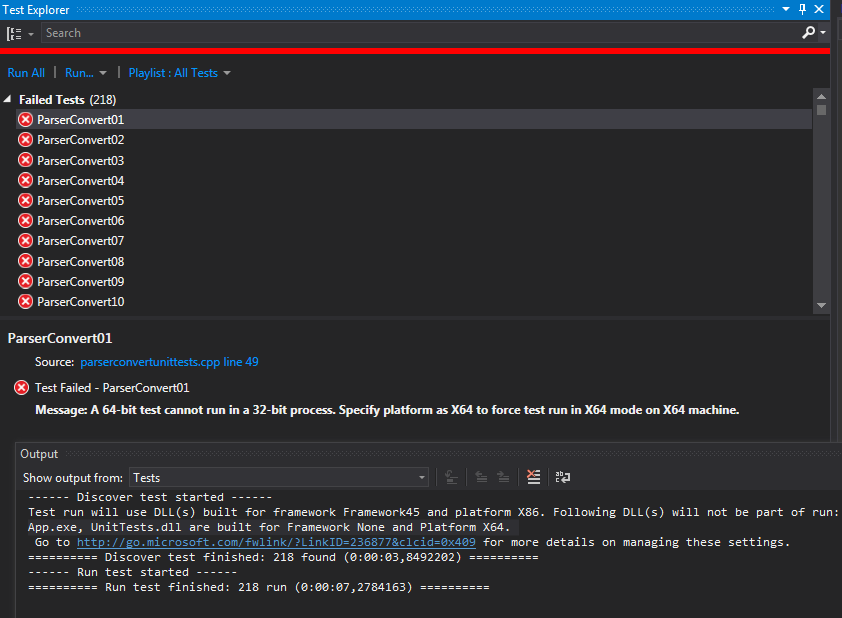
\includegraphics[width=15cm]{img/UnitTests_wrong_architecture.png}
	\caption{Uruchamienie testów jednostkowych na złej architekturze}
\end{figure}

By zmienić architekturę na 64-bit, należy przestawić jej wartość domyślną dla śodowiska testowego w sposób, w jaki zostało to przedstawione na rysunku niżej.

\begin{figure}[H]
	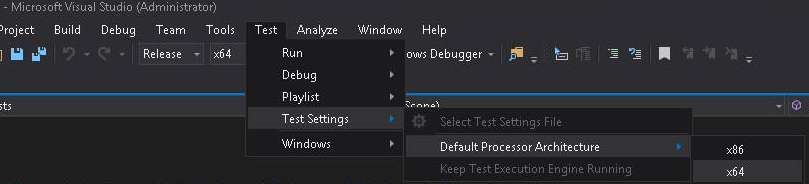
\includegraphics[width=15cm]{img/UnitTests_x64_architecture.png}
	\caption{Ustawienie domyślnej architektury środowiska testowego}
\end{figure}
